\section{Предлагаемое решение}
\label{sec:Chapter3} \index{Chapter3}


\subsection{Функции потерь}
\label{sec:LossFunctions}
    Теперь рассмотрим специфические для задачи построения эмбеддингов функции потерь \cite{weng2021contrastive}, предполагаемо улучшающие кластеризацию.

\subsubsection{Contrastive loss}

Contrastive loss \cite{LossContrstive} для каждой пары объектов $\left(x_i, x_j\right)$ минимизирует расстояние эмбеддингов, если они из одного класса, и максимизирует, если они из разных классов:


$\begin{aligned} \mathcal{L}_{\text {cont }}\left(\mathbf{x}_i, \mathbf{x}_j, \theta\right) = & \mathbb{1}\left[y_i=y_j\right]\left\|f_\theta\left(\mathbf{x}_i\right)-f_\theta\left(\mathbf{x}_j\right)\right\|_2^2+ \\ & \mathbb{1}\left[y_i \neq y_j\right] \max \left(0, \epsilon-\left\|f_\theta\left(\mathbf{x}_i\right)-f_\theta\left(\mathbf{x}_j\right)\right\|_2\right)^2\end{aligned}$


Где $\epsilon$ это гиперпараметр, определяющий минимальное расстояние между объектами разных классов.

\subsubsection{Triplet loss}
\begin{figure}[h!]
\caption{Схема работы Triplet Loss}
\centering
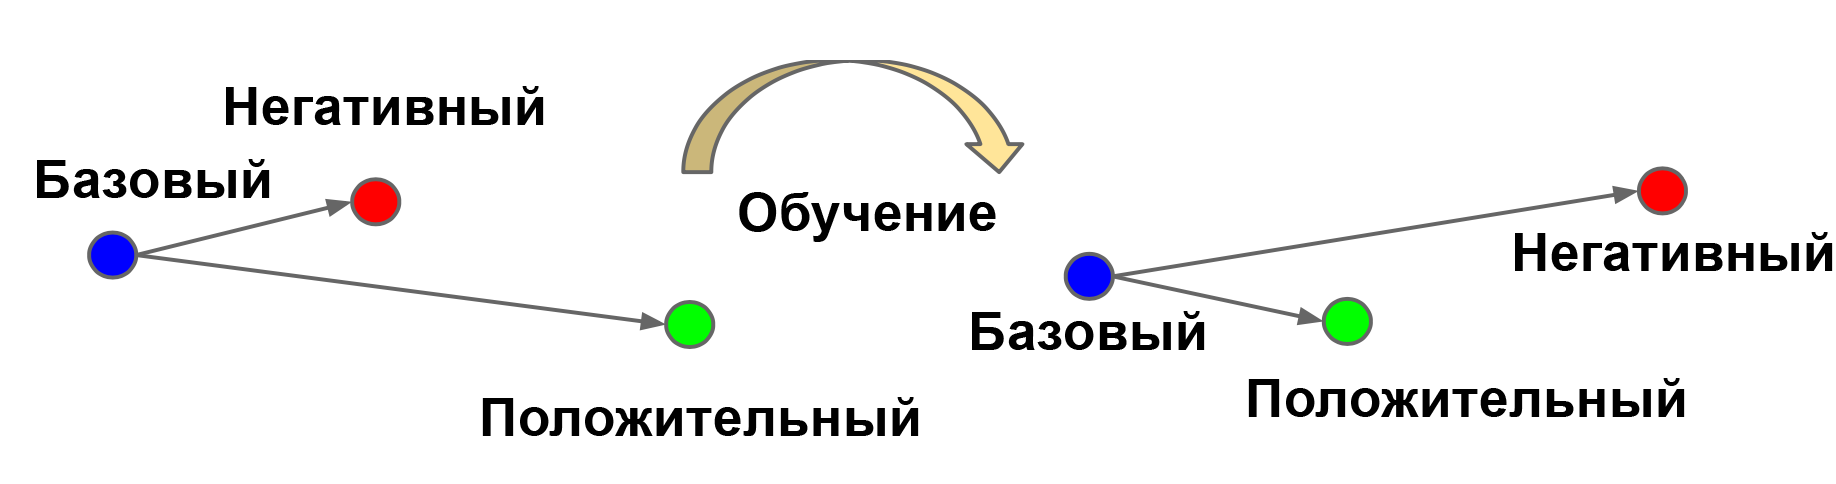
\includegraphics[width=16cm]{Images/triplet_loss_rus_noback.png}
\label{fig:triplet_loss_rus_noback}
\end{figure}

\label{img:TripletLoss}
    Triplet Loss \cite{LossTriplet} развивает идею Contrastive loss, но расчет идет сразу по трем объектам: базовый пример $\mathbf{x}$, положительный  пример (того же класса, что и базовый) $\mathbf{x}^{+}$ и один негативный пример (другого класса) $\mathbf{x}^{-}$. Triplet loss одновременно увеличивает расстояние между базовым и негативным объектами и уменьшает расстояние между базовым и положительным. (Рис \ref{fig:triplet_loss_rus_noback}):

\begin{center}
$$
\mathcal{L}_{\text {triplet }}\left(\mathbf{x}, \mathbf{x}^{+}, \mathbf{x}^{-}\right)=\sum_{\mathbf{x} \in \mathcal{X}} \max \left(0,\left\|f(\mathbf{x})-f\left(\mathbf{x}^{+}\right)\right\|_2^2-\left\|f(\mathbf{x})-f\left(\mathbf{x}^{-}\right)\right\|_2^2+\epsilon\right)
$$
\end{center}

\subsubsection{Lifted Structured loss}
Lifted Structured loss \cite{LossLifted} работает по тому же принципу, что и Triplet loss, однако он использует все пары объектов внутри одного тренировочного батча (Рис. \ref{fig:lifted_structured_loss_rus_noback}).

\begin{figure}[h!]
\caption{Сравнение функций потерь по выбору объектов}
\centering
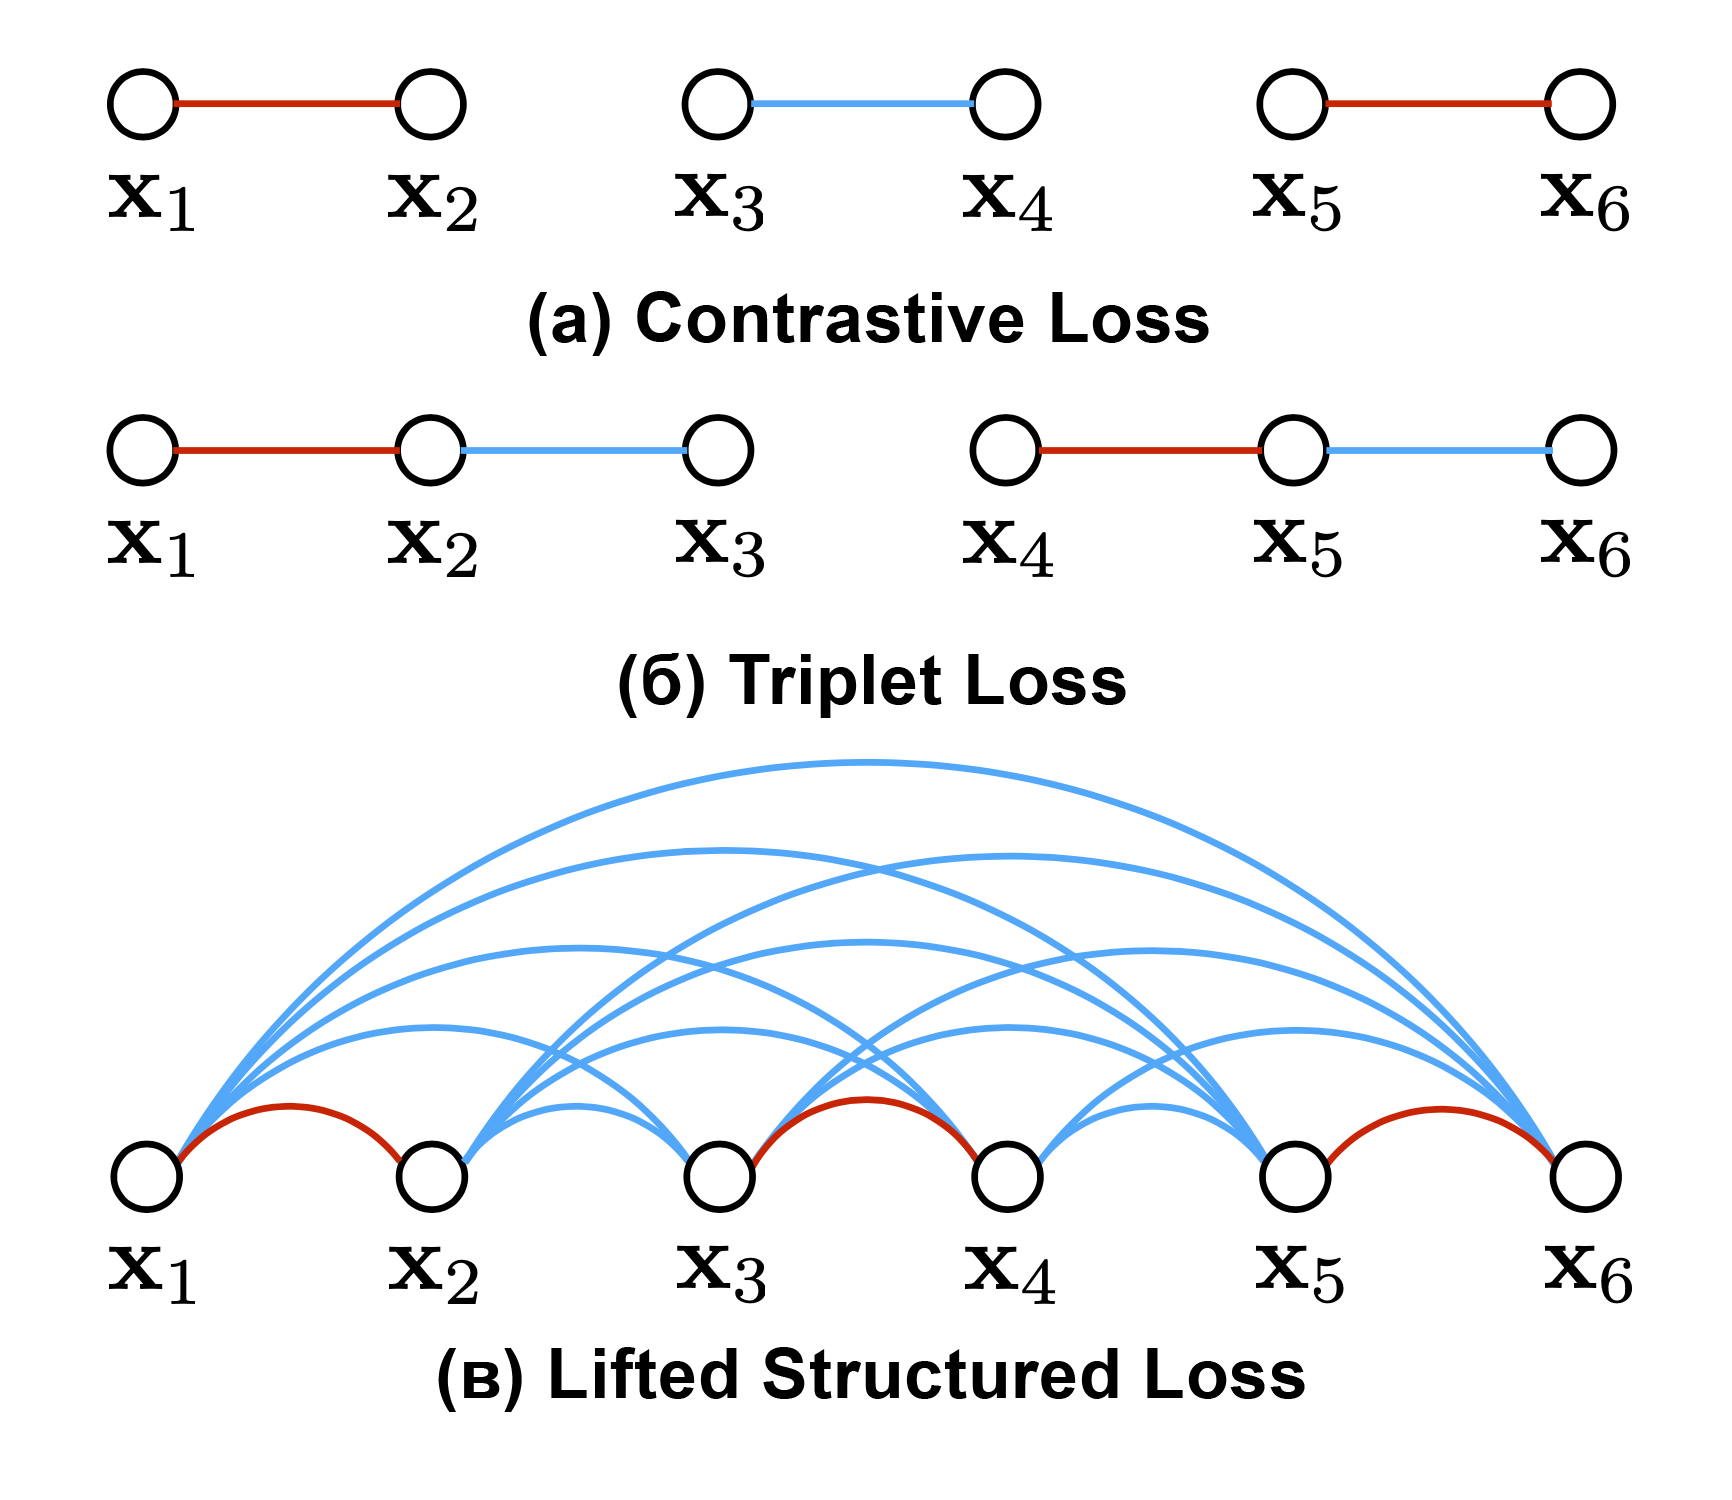
\includegraphics[width=16cm]{Images/lifted_structured_loss_rus_noback.png}
\label{fig:lifted_structured_loss_rus_noback}
\end{figure}


Пусть $D_{i j}=\left|f\left(\mathbf{x}_i\right)-f\left(\mathbf{x}_j\right)\right|_2$, $\mathcal{P}$ - набор положительных примеров, $\mathcal{N}$ - набор отрицательных примеров, тогда:

$$
\begin{aligned}
\mathcal{L}_{\text {struct }} & =\frac{1}{2|\mathcal{P}|} \sum_{(i, j) \in \mathcal{P}} \max \left(0, \mathcal{L}_{\text {struct }}^{(i j)}\right)^2 \\
\text { where } \mathcal{L}_{\text {struct }}^{(i j)} & =D_{i j}+\max \left(\max _{(i, k) \in \mathcal{N}} \epsilon-D_{i k}, \max _{(j, l) \in \mathcal{N}} \epsilon-D_{j l}\right)
\end{aligned}
$$

Правая часть в $\mathcal{L}_{\text {struct }}^{(i j)}$ призвана искать сложные негативные примеры (наиближайшие отрицательные примеры к базовому). Однако это функция ступенчатая, что может вызвать проблемы во время обучения, поэтому используют её сглаженную версию:

$$
\mathcal{L}_{\text {struct }}^{(i j)}=D_{i j}+\log \left(\sum_{(i, k) \in \mathcal{N}} \exp \left(\epsilon-D_{i k}\right)+\sum_{(j, l) \in \mathcal{N}} \exp \left(\epsilon-D_{j l}\right)\right)
$$

\subsubsection{N-pair loss}

N-pair loss \cite{LossNpair} -  это обобщение triplet loss, использующее не один, а несколько ($N-1$) негативных примеров. Таким образом, выбирается базовый пример, один положительный и ($N-1$) негативных примеров.
$$
\begin{aligned}
\mathcal{L}_{\mathrm{N}-\mathrm{pair}}&\left(\mathbf{x}, \mathbf{x}^{+},\left\{\mathbf{x}_i^{-}\right\})_{i=1}^{N-1}\right)  =\log \left(1+\sum_{i=1}^{N-1} \exp \left(f(\mathbf{x})^{\top} f\left(\mathbf{x}_i^{-}\right)-f(\mathbf{x})^{\top} f\left(\mathbf{x}^{+}\right)\right)\right) \\
& =-\log \frac{\exp \left(f(\mathbf{x})^{\top} f\left(\mathbf{x}^{+}\right)\right)}{\exp \left(f(\mathbf{x})^{\top} f\left(\mathbf{x}^{+}\right)\right)+\sum_{i=1}^{N-1} \exp \left(f(\mathbf{x})^{\top} f\left(\mathbf{x}_i^{-}\right)\right)}
\end{aligned}
$$

\begin{figure}[h!]
\caption{Формирование пакета для N-pair loss}
\centering
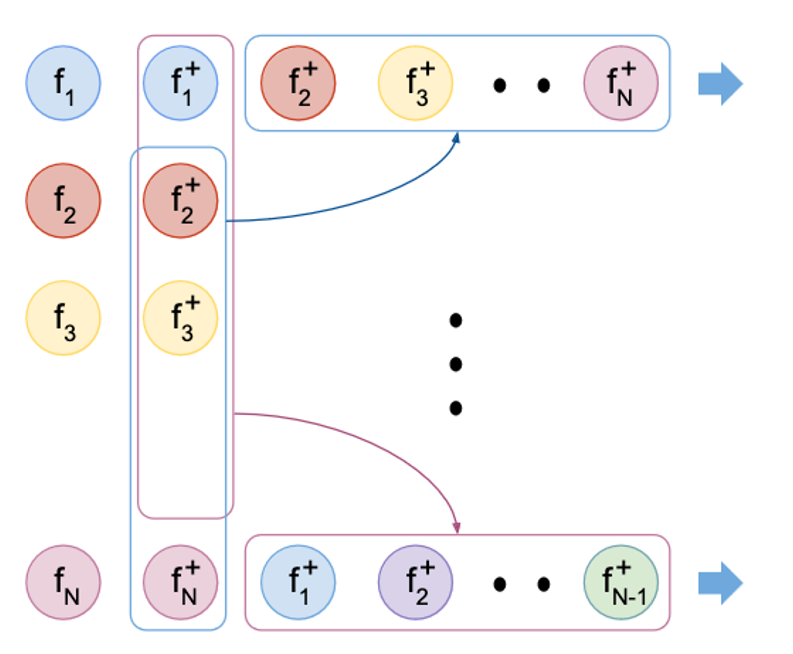
\includegraphics[width=12cm]{Images/N_pair_batch.png}
\label{fig:N_pair_batch}
\end{figure}

\subsection{Кластеризация}
    Как следует из цели подхода, основанного на построении эмбеддингов, исходные данные должны быть разделимы в новом пространстве. Это особенно важно для экстремальных случаев FSL: обучение по одному примеру (One Shot Learning или OSL) или обучение без примеров (Zero Shot Learning или ZSL). На Рис. \ref{fig:ClusteringGoodPoor} точками изображены экземпляры двух синтетических классов. Если кластеры достаточно удалены друг от друга, то нам не важно какие точки выбрать (какие примеры нам попадутся в обучающей выборке) для построения разделяющей гиперплоскости (в данном случае прямой), а если кластеры близки или вообще пересекаются, то качество разделяющей гиперплоскости будет зависеть от полученных примеров. Следовательно для оценки свойств полученного пространства будем вычислять метрики, характеризующие свойства  кластеризации данных.

    \begin{figure}[!ht]
      \begin{center}
          
      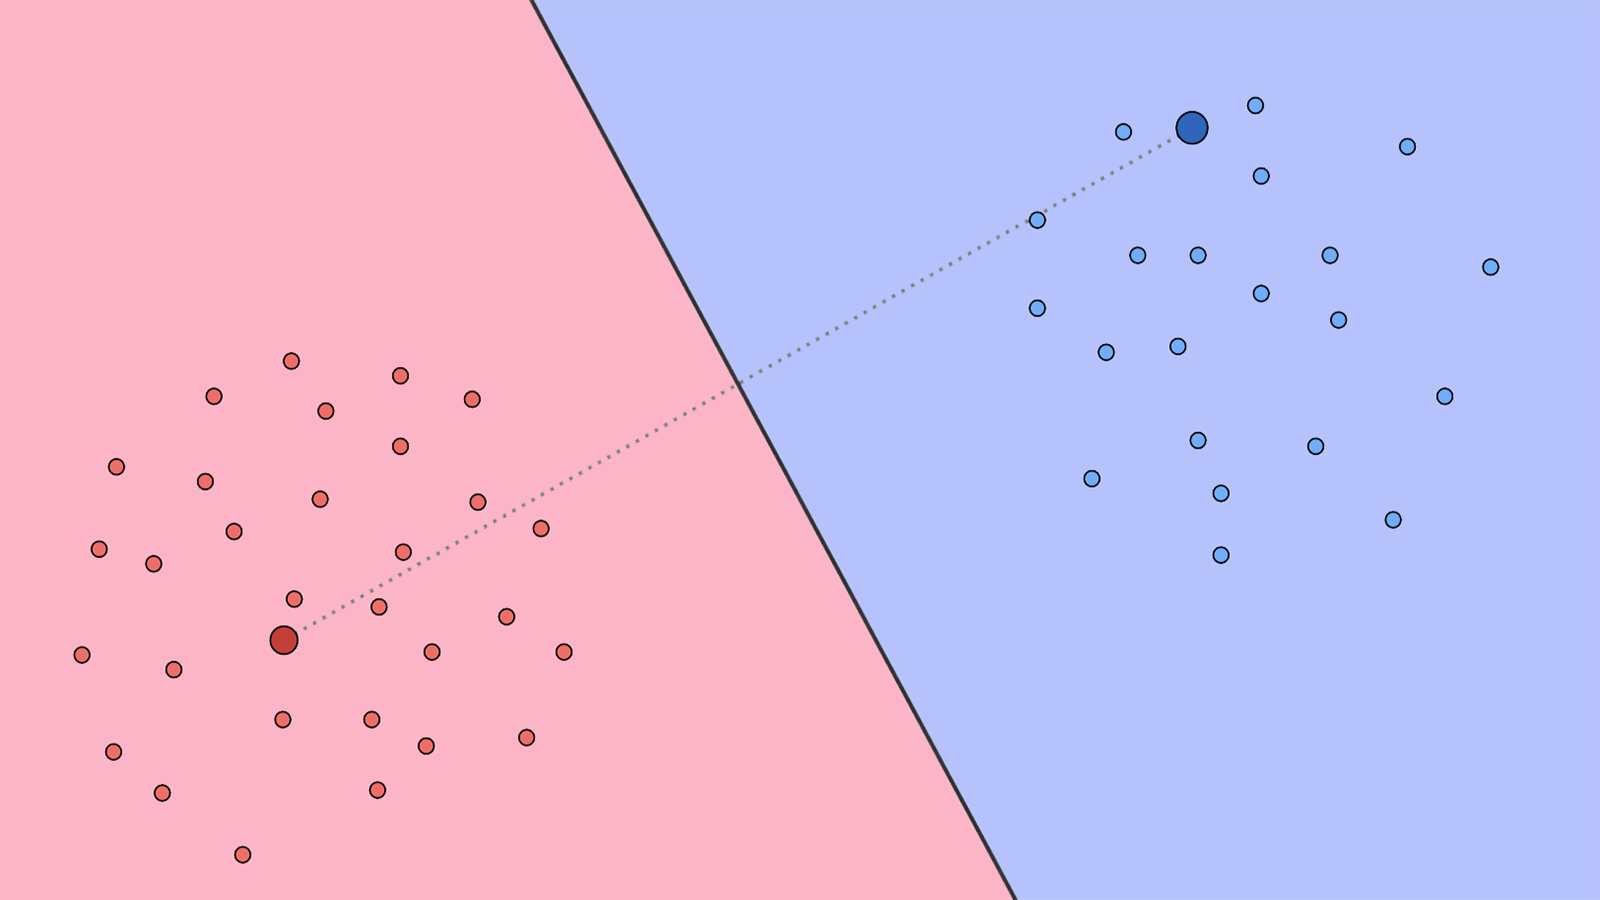
\includegraphics[width=10cm]{Images/good_clustering.png}
      \caption*{(a)}
      
      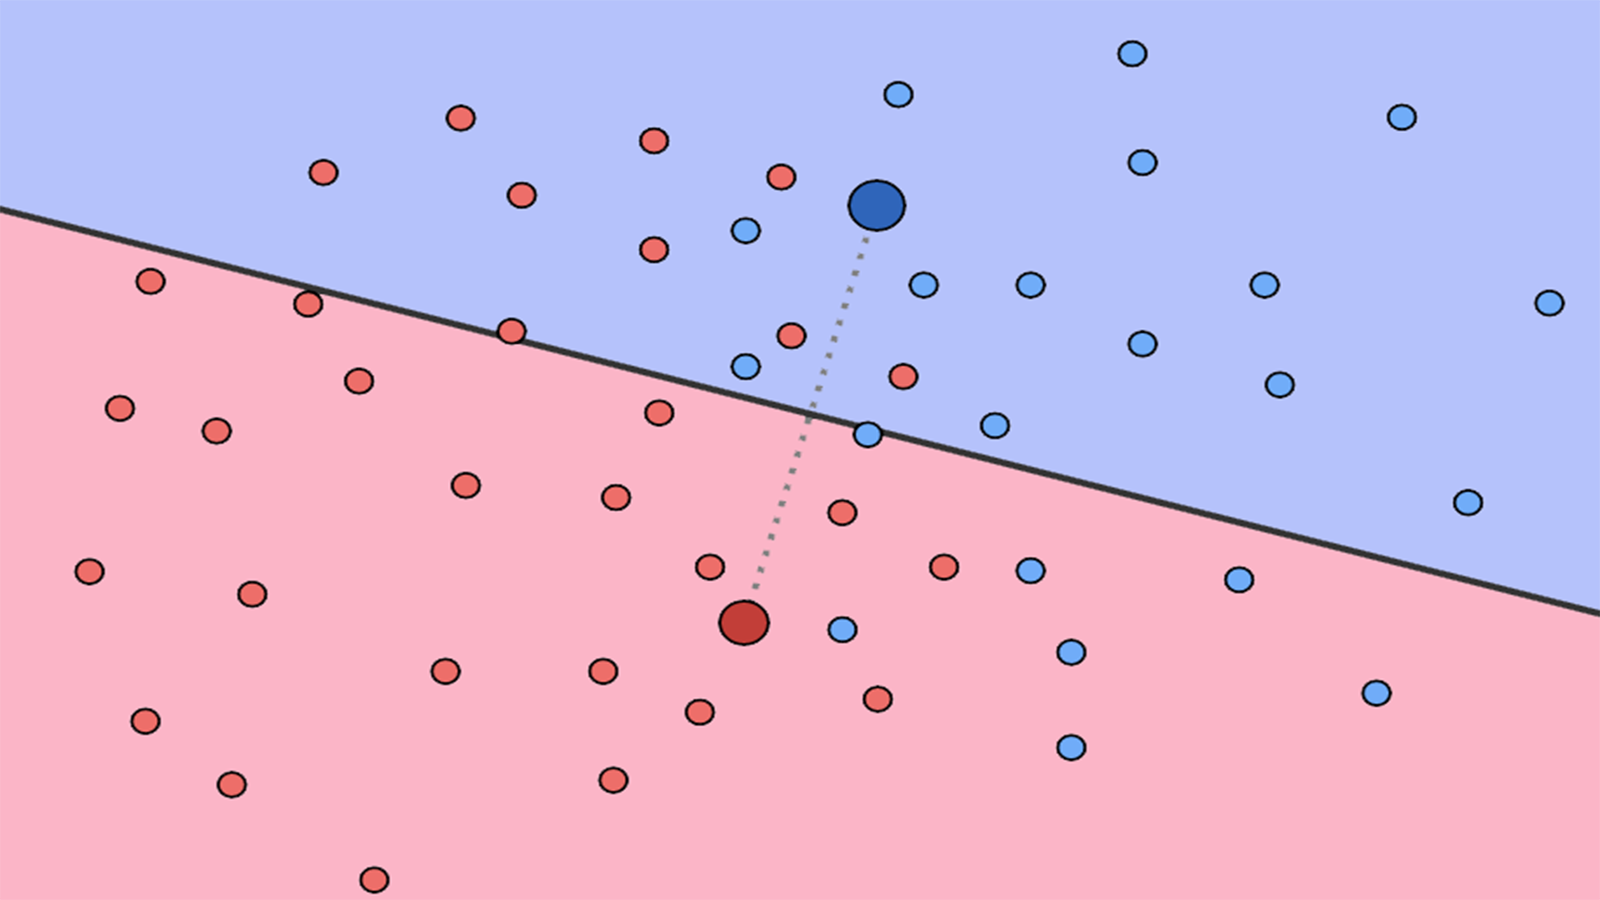
\includegraphics[width=10cm]{Images/poor_clustering.png}
      \caption*{(b)}      
      
      \end{center}
    \caption{Примеры хорошей (a) и плохой (b) класетризации}
    \label{fig:ClusteringGoodPoor}
    \end{figure}
    
\subsubsection{Оценка качества}
\label{subsec:ClusteringQuality}
    Для определения качества кластеризации вводятся следующие функции \cite{EmbedMetaFSL}:
    \begin{itemize}
        \item Отношение внутриклассовой к межклассовой дисперсии (intra-class to inter-class variance ratio): 
        \begin{center}
            
        \Large
        $R_{FC}=\frac{\sigma_{\text {within }}^2}{\sigma_{\text {between }}^2}=\frac{\frac{\sum_{i, j}\left\|\phi_{i, j}-\mu_i\right\|_2^2}{N}}{\frac{\sum_i\left\|\mu_i-\mu\right\|_2^2}{C}}=\frac{C}{N} \frac{\sum_{i, j}\left\|\phi_{i, j}-\mu_i\right\|_2^2}{\sum_i\left\|\mu_i-\mu\right\|_2^2}$,
        
        \end{center}
        \normalsize

        где $C$ - количество классов, $N$ - количество объектов в классе,  $\phi_{i, j}$ - эмбеддинг $j$-ого объекта в $i$-ом классе, $\mu_i$ - среднее эмбеддингов $i$-ого класса, $\mu$ - среднее эмбеддингов всех классов.
        Чем меньше значение полученного выражения, тем лучше кластеризация.

        \item Ограничение разброса гиперплоскостей: Пусть $x_1, x_2$ - объекта одного класса, $y_1, y_2$ - объекты другого класса, $f_\theta\left(x\right)$ - эмбеддинг объекта $x$, тогда выражение $f_\theta\left(x_1\right)-f_\theta\left(y_1\right)$ показывает направление разделяющей гиперплоскости с наибольшим зазором. Следующее выражение показывает насколько разные гиперплоскости можно построить, выбирая различные пары объектов из двух классов: 
        
        \begin{center}

        \Large
        
        $\begin{aligned} R_{HV} & \left(f_\theta\left(x_1\right), f_\theta\left(x_2\right), f_\theta\left(y_1\right), f_\theta\left(y_2\right)\right) \\ & =\frac{\left\|\left(f_\theta\left(x_1\right)-f_\theta\left(y_1\right)\right)-\left(f_\theta\left(x_2\right)-f_\theta\left(y_2\right)\right)\right\|_2}{\|\left(f_\theta\left(x_1\right)-f_\theta\left(y_1\right)\left\|_2+\right\| f_\theta\left(x_2\right)-f_\theta\left(y_2\right) \|_2\right.} .\end{aligned}$
        
        \end{center}
        \normalsize
        Как и в первом случае чем меньше значение $R_{H V}$, тем лучше кластеризация.
        
    \end{itemize}

\subsection{Тестовая задача}
Для проведения экспериментов выбрана задача распознавания ключевых слов (Keyword Spotting) на пример набора данных Google Speech V2 \cite{GoogleSpeechDataset}. Датасет представляет собой набор из 105,829 примеров для 35 различных английских слов. Каждый пример представляет собой аудио файл формата WAV, длительностью не более одной секунды. В записи участвовали 2618 людей. Также, помимо примеров самих слов, датасет предоставляет несколько файлов с фоновым шумом. 

На вход нейронной сети подается представление аудио файла в виде мел спектрограммы: в отличие от обыной спектрограммы используется нелинейная шкала частот, отображающая воприятие звука человеком. Так, для более низких частот получается больше делений (мелов), чем для высоких. В итоге, в качеств входа модели выступает двумерный массив, для которого естественно использовать сверточные нейронные сети.

\subsection{Тестовая модель}
В качестве базовой модели выбрана модификация светрочной нейронной сети под названием Depthwise Separable Convolution Neural Network (DS-CNN). В статье \cite{KeywordSpottingMicrocontrollers} проводилось сравнение различных моделей нейронных сетей на датасете Google Speech V1, в ходе которого DS-CNN показала наилучшую точность при сопоставимом числе операций. Общая структура DS-CNN модели представлена на Рис. \ref{fig:DS_CNN_model}. В ходе экспериметнов использовался вариант DS-CNN, включающий в себя 4 блока DS-Conv, каждый по 64 карты признака. Размерность пространства эмбеддингов (количество нейрнов после слоя Average Pool) также 64.

\begin{figure}[h!]
\caption{Структура DS-CNN}
\centering
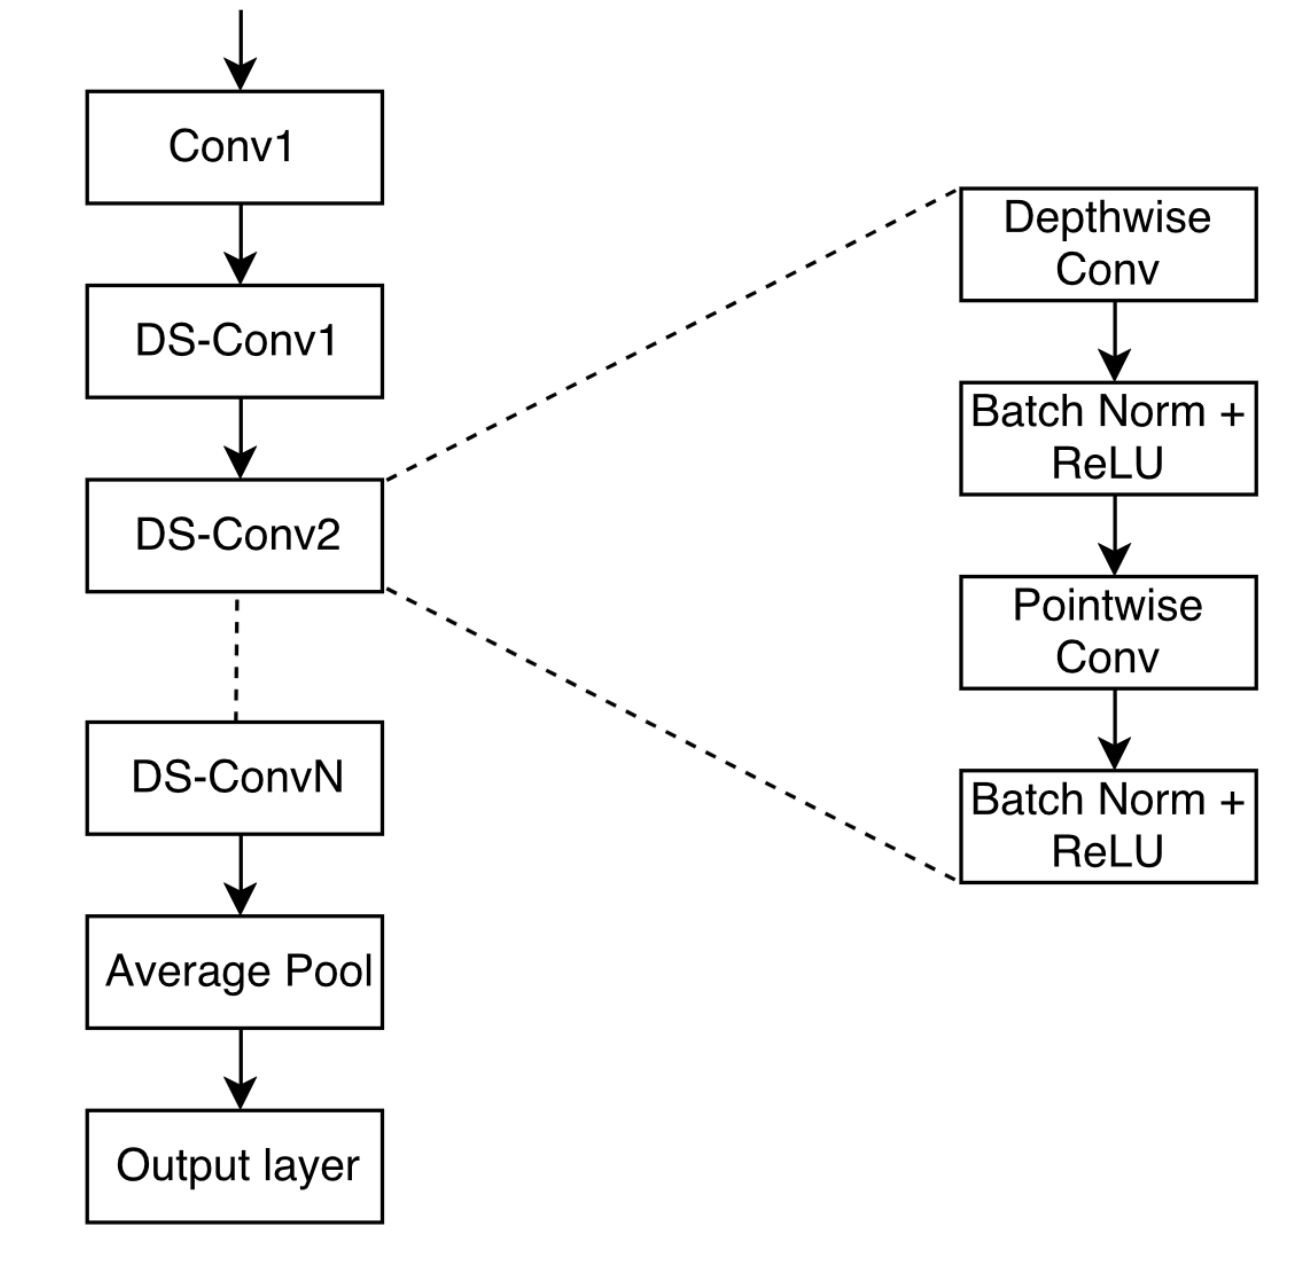
\includegraphics[width=16cm]{Images/DS_CNN_model.png}
\label{fig:DS_CNN_model}
\end{figure}